\section{การเรียนรู้เชิงลึก (Deep Learning)}
การเรียนรู้เชิงลึก (Deep Learning) คือความพยายามในการจำลองเซลล์ประสามของมนุษย์ให้อยู่ในรูปโมเดลคณิตศาสตร์
ด้วยความเชื่อทางหลักประสาทวิทยา (neurosciences) ว่าความฉลาดของสมองมนุษย์เกิดขึ้นได้จากโครงข่ายประสาทจำนวนมาก
ที่เชื่อมเข้าถึงกัน \cite{mit-dl}

\subsection{เปอร์เซปตรอน (Perceptron)}
\begin{figure}[h]
    \centering
    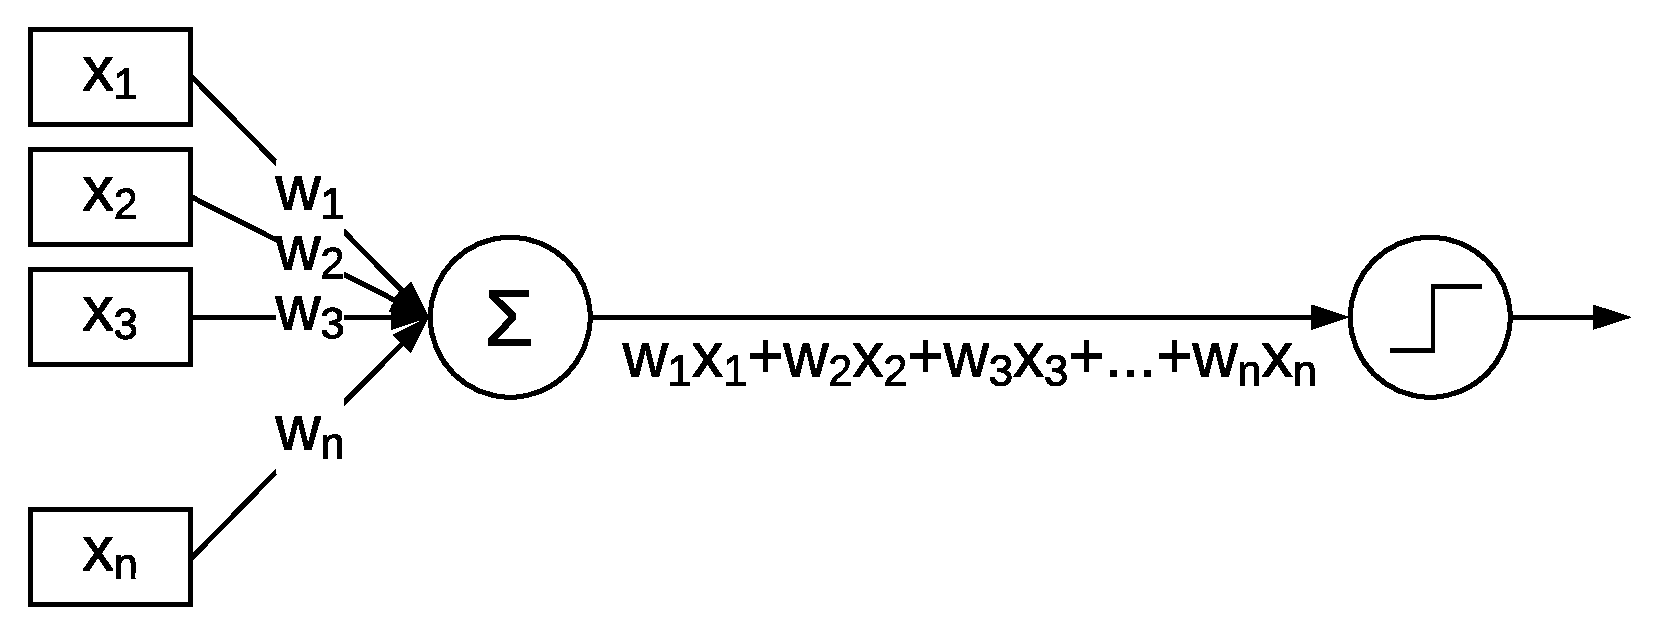
\includegraphics[width=0.7\textwidth]{images/perceptron.pdf}
    \caption{เปอร์เซปตรอน}
    \label{perceptron}
\end{figure}
เปอร์เซปตรอน (Perceptron) เป็นแบบจำลองทางคณิตศาสตร์ของเซลล์สมองหนึ่งเซลล์ โดยมีคุณสมบัติดังนี้

\begin{itemize}
    \item รับเข้าข้อมูลมาในเซลล์จากหลายแหล่ง และให้น้ำหนักกับข้อมูลนั้นต่างกันไป
    \item ส่งออกข้อมูลเพียงค่าเดียว
\end{itemize}

ดังนั้น แบบจำลองทางคณิตศาสตร์สามารถเขียนออกมาจากหลักการสองข้อดังกล่าวได้ด้วยสมการ

$$ y = f\left(W^TX+b\right) $$

เมื่อ $W$ และ $X$ เป็นเวกเตอร์ขนาด $1 \times n$ (โดย $n$ เป็นจำนวนข้อมูลรับเข้า), $b$ เป็นค่าสัมประสิทธิ์คงที่ (ไบแอส: bias)
และ $f$ เป็นฟังก์ชั่นกระตุ้น (activation function) ซึ่งอาจเขียนรูปร่างของเปอร์เซปตรอนให้มีลักษณะรูปคล้ายเซลล์สมองได้ในลักษณะรูปที่ \ref{perceptron}

ยกตัวอย่างการใช้เปอร์เซปตรอนในการแก้ปัญหาอย่างง่ายได้ในที่นี้

\subsubsection{การคาดเดาราคาอสังหาริมทรัพย์}
หากสำรวจราคาอสังหาริมทรัพย์แล้วพบว่า
\begin{itemize}
    \item ราคาอสังหาริมทรัพย์จะเพิ่มขึ้นตามที่ดิน โดยเพิ่มขึ้นทุก 10,000 บาทต่อตารางวา
    \item ราคาอสังหาริมทรัพย์จะเพิ่มขึ้นตามจำนวนห้องนอน โดยเพิ่มขึ้นทุก 200,000 บาทต่อห้องนอน
    \item ราคาอสังหาริมทรัพย์จะลดลงตามจำนวนอายุปี โดยลดลงทุก 7,000 บาทต่ออายุของอสังหาริมทัพย์
\end{itemize}
\noindent
จะสามารถเขียนเปอร์เซปตรอนเพื่อคาดเดาราคาอสังหาริมทรัพย์ได้โดย
$$ y = f\left(W^TX+b\right) $$
เมื่อ $W$ ซึ่งเป็นค่าสัมประสิทธิ์แสดงถึงความสัมพันธ์ข้อมูลรับเข้า ซึ่งเขียนได้จากความสัมพันธ์ดังแสดงด้านล่าง
$$
    W^T = \begin{bmatrix}
        10000 & 200000 & -7000
    \end{bmatrix}
$$
$b$ เป็นไบแอส, จะสมมติให้ $b = 0$ (กล่าวโดยละเอียด ในที่นี้ $b$ คือราคาตั้งต้นของบ้าน 0 ห้องนอน พื้นที่ 0 ตารางวา อายุ 0 ปี) และ $f(x) = x$ กล่าวคือเป็นฟังก์ชั่นเชิงเส้น

หากต้องการคาดเดาราคาบ้านที่มี 3 ห้องนอน เนื้อที่ 100 ตารางวา และมีอายุ 7 ปี จะสามารถเขียนเวกเตอร์ $P$ ได้เป็น

$$
    X = \begin{bmatrix}
        3 \\
        100 \\
        7
    \end{bmatrix}
$$
และผลการทำนายราคาบ้านคำนวนได้จาก
$$
    \begin{aligned}
        y &= f\left(W^TX+b\right)\\
        &= f\left(\begin{bmatrix}
            10000 & 200000 & -7000
        \end{bmatrix} \times \begin{bmatrix}
            3 \\
            100 \\
            7
        \end{bmatrix}\right)\\
        &= f(30000 + 20000000 + (-49000)) = f(19981000)\\
        &= 19981000
    \end{aligned}
$$

\subsubsection{การสร้างประตูสัญญาณตรรกะด้วยเปอร์เซปตรอน}
เราสามารถสร้างประตูสัญญาณตรรกะ (logic gates) บางชนิดได้ด้วยเปอร์เซปตรอน เช่นการสร้าง AND และ OR gate

ยกตัวอย่างโครงสร้างของ AND gate ซึ่งสามารถสร้างได้ด้วยการกำหนดให้
\begin{itemize}
    \item $X$ เป็นเมทริกซ์ขนาด $1 \times 2$ กล่าวคือเมื่อรับค่า $x_1, x_2$ เป็นค่า 0 หรือ 1 แทนสัญญาณจริงหรือเท็จแล้ว
        $$X = \begin{bmatrix}
            a_1 \\
            a_2
        \end{bmatrix}$$
    \item กำหนดค่าของเมทริกซ์ $W$ เป็น
        $$W^T = \begin{bmatrix}
            1 && 1
        \end{bmatrix}$$
    \item กำหนดค่าของไบแอส $b = -2$
    \item กำหนดฟังก์ชั่น $f(x)$ เป็น step function กล่าวคือ
    $$
        f(x) = \begin{cases}
            1; & x \geq 0\\
            0; & \textrm{ในกรณีอื่น}
        \end{cases}
    $$
\end{itemize}
และการสร้าง OR gate สามารถทำได้ในลักษณะเดียวกันโดยเปลี่ยน $b$ เป็น $b = -1$

\subsection{เปอร์เซปตรอนแบบหลายชั้น (Multi Layer Perceptron)}

เราอาจสังเกตว่าเปอร์เซพตรอนหนึ่งตัวนั้นทำหน้าที่ได้เพียนแยก (classify) หรือถดถอย (regress) ปัญหาที่เป็นปัญหาเชิงเส้น (linear problems) ได้เท่านั้น อย่างไนก็ตามหากเรากำหนดให้ฟังก์ชั่น $f$ เป็นฟังก์ชั่นที่ไม่ใช่ฟังก์ชั่นเส้นตรงแล้ว เราอาจสร้าง\textbf{เปอร์เซปตรอนแบบหลายชั้น} (Multi Layer Perceptron) ขึ้นมาได้โดยมีลักษณะดังรูปที่ \ref{mlp}

\begin{figure}
    \centering
    \def\layersep{2.5cm}
    \begin{tikzpicture}[->,draw=black!70, node distance=\layersep]
        \tikzstyle{every pin edge}=[<-,shorten <=1pt]
        \tikzstyle{neuron}=[circle,draw=black!100,minimum size=17pt, outer sep=3pt]
        \tikzstyle{annot}=[text width=5em, text centered]
    
        \foreach \name / \y in {1,...,4}
            \node[neuron, pin=left:ข้อมูลรับเข้า \y] (I-\name) at (0,-\y) {};
    
        % Draw the hidden layer nodes
        \foreach \name / \y in {1,...,5}
            \path[yshift=0.5cm]
                node[neuron] (HA-\name) at (\layersep,-\y cm) {};
    
        \foreach \name / \y in {1,...,5}
            \path[yshift=0.5cm]
                node[neuron] (HB-\name) at (2*\layersep,-\y cm) {};

        \foreach \name / \y in {1,...,3}
            \path[yshift=-0.5cm]
                node[neuron] (O-\name) at (3*\layersep,-\y cm) {};
    
        \foreach \source in {1,...,4}
            \foreach \dest in {1,...,5}
                \path (I-\source) edge (HA-\dest);
    
        \foreach \source in {1,...,5}
            \foreach \dest in {1,...,5}
                \path (HA-\source) edge (HB-\dest);

        \foreach \source in {1,...,5}
            \foreach \dest in {1,...,3}
                \path (HB-\source) edge (O-\dest);

        \node[annot,above of=I-1, node distance=1cm] (hla) {ชั้นรับเข้า (ชั้นที่ 0)};
        \node[annot,above of=HA-1, node distance=1cm] (hla) {ชั้นซ่อน 1};
        \node[annot,above of=HB-1, node distance=1cm] (hla) {ชั้นซ่อน 2};
        \node[annot,above of=O-1, node distance=1cm] (hlb) {ชั้นส่งออก (ชั้นที่ 3)};
    \end{tikzpicture}
    \caption{เปอร์เซปตรอนแบบหลายชั้น}
    \label{mlp}
\end{figure}

เราอาจเขียนแทนน้ำหนักของโครงข่ายจากเปอร์เซปตรอนชั้นที่ $i$ ไปยังชั้นที่ $j$ ($j=i+1$) ได้เป็น
\begin{equation*}
    \boldsymbol{W}_{ij} = 
    \begin{bmatrix}
        w_{11} & w_{21} & \dots & w_{n_{i}1}\\
        w_{12} & w_{22} & \dots & w_{n_{i}2}\\
        \vdots & \vdots & \ddots & \vdots\\
        w_{1n_j} & w_{2n_j} & \dots & w_{n_jn_i}
    \end{bmatrix}
\end{equation*}
เมื่อจำนวนเปอร์เซปตรอนในชั้นที่ $k$ เขียนแทนด้วย $n_k$

ยกตัวอย่างเช่น เราจะสามารถสร้างประตูสัญญาณ XOR (XOR gate) ได้จากเปอร์เซปตรอนแบบหลายชั้นดังแสดงในรูปที่ \ref{xor-mlp} โดยเลขในแต่ละเปอร์เซปตรอนแทนค่าไบแอส ($b$) และเลขบนเส้นเชื่อมแทนค่าน้ำหนัก ($w$) และกำหนดให้ฟังก์ชั่นกระตุ้น $f$ เป็นฟังก์ชั่นขั้นบันได (step function) กล่าวคือ
\begin{equation*}
    f(x) =
    \begin{cases}
        1; & x \geq 0\\
        0; & \textrm{ในกรณีอื่น}
    \end{cases}
\end{equation*}
เปอร์เซปตรอนดังกล่าว เมื่อรับค่า $A$ และ $B$ เป็น 0 หรือ 1 จะส่งออกค่า $A \oplus B$

\begin{figure}
    \def\layersep{2.5cm}
    \centering
    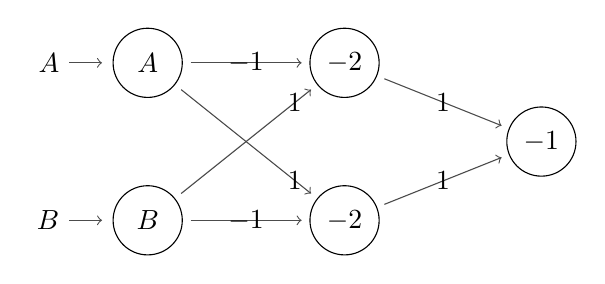
\begin{tikzpicture}[<-, draw=black!70, node distance=\layersep]
        \tikzstyle{edge}=[->,fill=white]
        \tikzstyle{neuron}=[circle,draw=black!100,minimum size=25pt, outer sep=3pt]
        \tikzstyle{annot}=[text width=5em, text centered]
    
        \node[neuron, pin=left:$A$] (I-1) at (0,0 cm) {$A$};
        \node[neuron, pin=left:$B$] (I-2) at (0,-2 cm) {$B$};
    
        \node[neuron] (HA-1) at (\layersep,-0 cm) {$-2$};
        \node[neuron] (HA-2) at (\layersep,-2 cm) {$-2$};

        \node[neuron] (O) at (2*\layersep,-1 cm) {$-1$};

        \path[edge]
            (I-1) edge node {$-1$} (HA-1)
            (I-1) edge node[very near end] {$1$} (HA-2)
            (I-2) edge node[very near end] {$1$} (HA-1)
            (I-2) edge node {$-1$} (HA-2)
            (HA-1) edge node {$1$} (O)
            (HA-2) edge node {$1$} (O)
        ;
    \end{tikzpicture}
    \caption{เปอร์เซปตรอนแบบหลายชั้นซึ่งทำหน้าที่เป็นประตูสัญญาณ XOR}
    \label{xor-mlp}
\end{figure}